\documentclass[20pt, a0paper, landscape]{tikzposter}
% \usepackage[utf8]{inputenc}
 
\title{OPTIMAL FISHING RATES FOR MULTIPLE FLEETS}
\author{Steven Martell and Catarina Wor}
\date{\today}
\institute{INTERNATIONAL PACIFIC HALIBUT COMMISSION}
 
\usepackage{blindtext}
\usepackage{comment}

% Themes
\usetheme{Default} 
\usetheme{Rays} 
% \usetheme{Basic} 
% \usetheme{Simple} 
% \usetheme{Envelope} 
% \usetheme{Wave} 
% \usetheme{Board} 
% \usetheme{Autumn} 
% \usetheme{Desert} 


% Block styles
\useblockstyle{Default}
\useblockstyle{Basic}
\useblockstyle{Minimal}
\useblockstyle{Envelope}
\useblockstyle{Corner}
\useblockstyle{Slide} 
\useblockstyle{TornOut}



% additional packages
% \usepackage{times}
\usepackage{amsmath,amsthm, amssymb, latexsym, bm}
% \usepackage{exscale}
% \usepackage{ragged2e}
% \boldmath
% \usepackage{booktabs, array}
% \usepackage{rotating} %sideways environment
\usepackage[english]{babel}
\usepackage[latin1]{inputenc}
% \listfiles
% \graphicspath{{figures/}}
% \graphicspath{{FIGS/}}




% abbreviations
\usepackage{xspace}
\makeatletter
\DeclareRobustCommand\onedot{\futurelet\@let@token\@onedot}
\def\@onedot{\ifx\@let@token.\else.\null\fi\xspace}
\def\eg{{e.g}\onedot} \def\Eg{{E.g}\onedot}
\def\ie{{i.e}\onedot} \def\Ie{{I.e}\onedot}
\def\cf{{c.f}\onedot} \def\Cf{{C.f}\onedot}
\def\etc{{etc}\onedot}
\def\vs{{vs}\onedot}
\def\wrt{w.r.t\onedot}
\def\dof{d.o.f\onedot}
\def\etal{{et al}\onedot}
\makeatother

\newcommand{\fspr}{F$_{\rm{SPR=35\%}}$}
\newcommand{\bspr}{B$_{\rm{SPR=35\%}}$}
\newcommand{\rspr}{R$_{\rm{SPR=35\%}}$}
\newcommand{\fofl}{F$_{\rm{OFL}}$}

\usepackage{pifont}% http://ctan.org/pkg/pifont
\newcommand{\cmark}{\ding{51}}%
\newcommand{\xmark}{\ding{55}}%

\newcommand{\fmsy} {F$_{\rm{MSY}}$}

\newcommand{\dye}  { \dfrac{{\partial y_k}}{{\partial f_k}} }%
\newcommand{\dre}  { \dfrac{{\partial R_e}}{{\partial f_k}} }%
\newcommand{\dphi} { \dfrac{{\partial \phi_k}}{{\partial f_k}} }%

\newcommand{\ddye}{ \dfrac{{\partial y_k}^2}{{\partial f_k}^2} }%
\newcommand{\ddre}{ \dfrac{{\partial R_e}^2}{{\partial f_k}^2} }%
\newcommand{\ddphi}{ \dfrac{{\partial \phi_k}^2}{{\partial f_k}^2} }%


\definecolor{cM1}{rgb}{0.9608,0.4706,0.4392}
\definecolor{cM2}{rgb}{0.4902,0.6745,0.1216}
\definecolor{cM3}{rgb}{0.2275,0.7765,0.7922}
\definecolor{cM4}{rgb}{0.7765,0.5020,0.9843}


\begin{document}
 
\maketitle
 
\block{~}
{
    \blindtext

    $x = \int f(x)$
}

\begin{columns}
    \column{0.4}
    \block{More text}{Text and more text \blindtext}
 
    \column{0.6}
    % \useblockstyle{Slide} 
    \block{Something else}{Here, \blindtext \vspace{4cm}}
    \note[
        targetoffsetx=-9cm, 
        targetoffsety=-16.5cm, 
        width=0.35\linewidth
        ]
        {e-mail \texttt{stevem@iphc.int}\\
        
        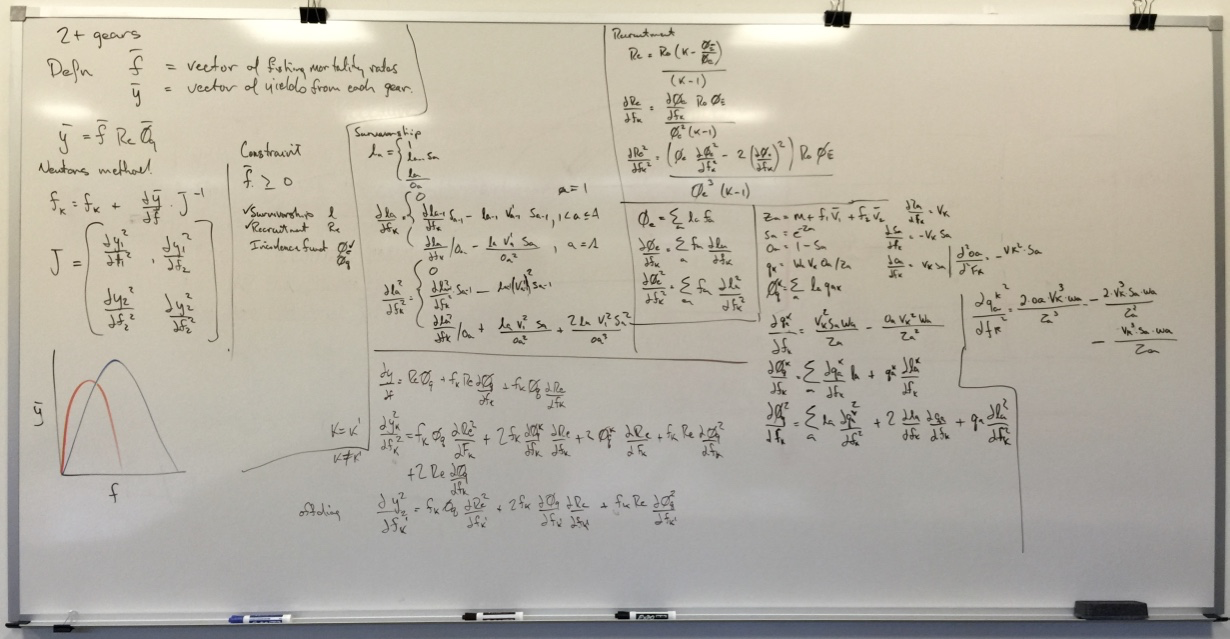
\includegraphics[width=0.95\linewidth,keepaspectratio=true]{./whiteBoard.png}}

\end{columns}

\begin{columns}
	\column{0.15}
	% \useblockstyle{Minimal} 
	\block{Symbols}{
		\begin{tabular}{cl}
			$\vec{f}$     & instantaneous fishing mortality rates.\\
			$\vec{y}$     & equilibrium yields.\\
			$\vec{\phi}$  & yield per recruit.\\
		\end{tabular}
	}

	\column{0.30}
	\block{Catch Equation And Finding \fmsy}{
		Assuming all fisheries and natural mortality operate simultaneously, the equilibrium catch equation for each fleet can be written as a vector
		\begin{align}
			%
			\vec{y} = \vec{f} R_e \vec{\phi}  \label{eq.1}
			%
		\end{align}
		To find the vector of fishing mortality rates that simultaneously maximizes the yield for each fleet we use Newton's method to find the solution to $\dfrac{\partial \vec{y}}{\partial \vec{f}} = 0$.  The first and second derivatives of \eqref{eq.1} for fleet $k$ are given by:
		\begin{align}
			%
			\dye &= R_e \phi_k
			+ f_k R_e \dphi
			+ f_k \phi \dre \\[1ex] \label{eq.2}
			%
			\mbox{Jacobian} \nonumber \\
			\ddye &=
			\begin{cases}
				f_k \phi \ddre + 2 f_k \dphi \dre + 2 \phi_k \dre + f_k R_e \ddphi + 2 R_e \dphi & k = k \\[2ex]
				%
				f_{k'} \phi \ddre + 2 f_{k'} \dphi \dre + f_{k'} R_e \ddphi & k \neq k'
			\end{cases} \label{eq.3}
		\end{align}
		The Newtons iteration step is given by:
		\begin{align}
			\vec{f}_{i+1} = \vec{f}_{i} - \dfrac{\partial y}{\partial f}
			 \left( \dfrac{{\partial y}^2}{{\partial f}^2} \right)^{-1}
		\end{align}
	}% end block.
\end{columns}

\end{document}